\documentclass[12pt]{article}
\usepackage[12pt]{moresize}
\usepackage[margin=1in]{geometry}

\usepackage{amsmath}
\usepackage{amssymb}

\usepackage{graphicx}
\usepackage{subcaption}

\usepackage{multirow} %Combining rows in tables
\usepackage{diagbox}  %Table box split in twain

\usepackage{algorithm}
\usepackage{algpseudocode}
\usepackage{alltt}

\usepackage{multicol}

\usepackage{amssymb} %\checkmark symbol

%\usepackage{hyperref}
%\usepackage[latin1]{inputenc}
%\usepackage{listings}
%\usepackage{scrextend}
%\usepackage{changepage} %Adjustwidth

  

\title{ComS 472\\Homework 4}
\author{Sean Gordon}
\date{Oct 26, 2020}

\begin{document}
\maketitle

\ \\
\centerline{- 7.22 - }
\ \\
\noindent 1) If the pair of clauses has no complimentary literals, there are no resolvents. \checkmark\\[.4em]
\indent If the pair has one or more sets of complimentary literals, the resulting resolvents \\
\indent acquired from applying the same set of literals in any order will eventually reduce\\
\indent down to a single resolvent. \checkmark\\

\noindent 2) A clause resolved with itself would contain complimentary literals left in the equation.\\
\indent As this clause does not contain any, it is impossible.\\[.4em]

\noindent 3) For a clause to resolve with a copy of itself, it must contain only complimentary \\[.4em]
\indent literals. This would make the initial clause equivalent to True\\[.4em]



\noindent \hrulefill \pagebreak



\centerline{- 7.23 - }
\ \\
\noindent 1) 
\begin{tabular}{|c|c|c||c|c|c||c|c||c|}
	\hline &&&&&&&&\\[-1em]
F & P & D &  F $\Rightarrow$ P  &  D $\Rightarrow$ P  & (F $\Rightarrow$ P)$\vee$  &  F $\wedge$ D  &  (F $\wedge$ D) & (F $\Rightarrow$ P)$\vee$(D $\Rightarrow$ P)\\
 & & & & & (D $\Rightarrow$ P) & &  $\Rightarrow$ P & $\Rightarrow$ (F $\wedge$ D)$\Rightarrow$ P\\
	\hline &&&&&&&&\\[-1em]
	\hline &&&&&&&&\\[-1em]
T&T&T&T&T&T&T&T&T \\
	\hline &&&&&&&&\\[-1em]
T&T&F&T&T&T&F&T&T \\
	\hline &&&&&&&&\\[-1em]
T&F&T&F&F&F&T&F&T \\
	\hline &&&&&&&&\\[-1em]
T&F&F&F&T&T&F&T&T \\
	\hline &&&&&&&&\\[-1em]
F&T&T&T&T&T&F&T&T \\
	\hline &&&&&&&&\\[-1em]
F&T&F&T&T&T&F&T&T \\
	\hline &&&&&&&&\\[-1em]
F&F&T&T&F&T&F&T&T \\
	\hline &&&&&&&&\\[-1em]
F&F&F&T&T&T&F&T&T \\
	\hline
\end{tabular}\\
\begin{center}\textbf{The sentence is valid as it is true for all combinations of variables.}\\[.4em]\end{center}

\noindent 2) Original\indent \indent\indent\ (F $\Rightarrow$ P)$\vee$(D $\Rightarrow$ P) $\Rightarrow$ (F $\wedge$ D)$\Rightarrow$ P\\[.4em]
\indent Implication Elim: ($\neg$F $\vee$ P)$\vee$ (D $\Rightarrow$ P) $\Rightarrow$ (F $\wedge$ D) $\Rightarrow$ P\\
\indent Implication Elim: ($\neg$F $\vee$ P)$\vee$ ($\neg$D $\vee$ P) $\Rightarrow$ (F $\wedge$ D) $\Rightarrow$ P\\
\indent Implication Elim: ($\neg$F $\vee$ P)$\vee$ ($\neg$D $\vee$ P) $\Rightarrow$ $\neg$(F $\wedge$ D) $\vee$ P\\
\indent De Morgan: \indent\ \ \ ($\neg$F $\vee$ P) $\vee$ ($\neg$D $\vee$ P) $\Rightarrow$ ($\neg$F $\vee$ $\neg$D) $\vee$ P\\
\indent Implication Elim: $\neg$(($\neg$F $\vee$ P )$\vee$ ($\neg$D $\vee$ P)) $\vee$ ($\neg$F $\vee$ $\neg$D)$\vee$ P\\
\indent De Morgan: \indent\ \ \ $\neg$($\neg$F $\vee$ P)$\wedge$ $\neg$($\neg$D $\vee$ P) $\vee$ ($\neg$F $\vee$ $\neg$D)$\vee$ P\\
\indent De Morgan: \indent\ \ \ (F $\wedge$ $\neg$P) $\wedge$ (D $\wedge$ $\neg$P) $\vee$ ($\neg$F $\vee$ $\neg$D)$\vee$ P\\
\indent Associativity: \indent\ (F $\wedge$ $\neg$P $\wedge$ D $\wedge$ $\neg$P) $\vee$ ($\neg$F $\vee$ $\neg$D $\vee$ P)\\
\indent Duplicates:\indent\indent\ (F $\wedge$ $\neg$P $\wedge$ D) $\vee$ ($\neg$F $\vee$ $\neg$D $\vee$ P)\\

\indent Final Form (CNF): \textbf{(F $\wedge$ $\neg$P $\wedge$ D) $\vee$ ($\neg$F $\vee$ $\neg$D $\vee$ P)}\\

\noindent 3) 
\begin{tabular}{|c|c|c||c|c|c||c||c||c|}
	\hline &&&&&&&&\\[-1em]
F & P & D &  $\neg$F  &  $\neg$P  &  $\neg$D  &  F $\wedge$ $\neg$P $\wedge$ D  &  $\neg$F $\vee$ P $\vee$ $\neg$D & F $\wedge$ $\neg$P $\wedge$ D  $\vee$  $\neg$F $\vee$ P $\vee$ $\neg$D\\
	\hline &&&&&&&&\\[-1em]
	\hline &&&&&&&&\\[-1em]
T&T&T&F&F&F&F&T&T\\
	\hline &&&&&&&&\\[-1em]
T&T&F&F&F&T&F&T&T\\
	\hline &&&&&&&&\\[-1em]
T&F&T&F&T&F&T&F&T\\
	\hline &&&&&&&&\\[-1em]
T&F&F&F&T&T&F&T&T\\
	\hline &&&&&&&&\\[-1em]
F&T&T&T&F&F&F&T&T\\
	\hline &&&&&&&&\\[-1em]
F&T&F&T&F&T&F&T&T\\
	\hline &&&&&&&&\\[-1em]
F&F&T&T&T&F&F&T&T\\
	\hline &&&&&&&&\\[-1em]
F&F&F&T&T&T&F&T&T\\
	\hline
\end{tabular}\\
\begin{center}\textbf{The resolved sentence is logically equivalent to the original.}\\[.4em]\end{center}



\noindent \hrulefill \\



\centerline{- 7.26 - }
\ \\
\noindent S1) A $\Leftrightarrow$ (C $\vee$ E) to...\\
\indent (A $\Rightarrow$ (C $\vee$ E)) $\wedge$ ((C $\vee$ E) $\Rightarrow$ A)\\
\indent ($\neg$A $\vee$ (C $\vee$ E)) $\wedge$ ($\neg$(C $\vee$ E) $\vee$ A)\\
\indent ($\neg$A $\vee$ C $\vee$ E) $\wedge$ (($\neg$C $\wedge$ $\neg$E) $\vee$ A)\\
\indent ($\neg$A $\vee$ C $\vee$ E) $\wedge$ ($\neg$C $\vee$ A) $\wedge$ ($\neg$E $\vee$ A)\\[.4em]

\noindent S2) E $\Rightarrow$ D to...\\
\indent $\neg$E $\vee$ D\\[.4em]

\noindent S3) B $\wedge$ F $\Rightarrow$ $\neg$C to...\\
\indent $\neg$(B $\wedge$ F) $\vee$ $\neg$C\\
\indent $\neg$B $\vee$ $\neg$F $\vee$ $\neg$C\\[.4em]

\noindent S4) E $\Rightarrow$ C to...\\
\indent $\neg$E $\vee$ C\\[.4em]

\noindent S5) C $\Rightarrow$ F to...\\
\indent $\neg$C $\vee$ F\\[.4em]

\noindent S6) C $\Rightarrow$ B to...\\
\indent $\neg$C $\vee$ B\\[.4em]



\noindent \hrulefill \\



\centerline{- 8.11 - }
\ \\
\noindent 1) Occupation(Emily, Surgeon) $\vee$ Occupation(Emily, Lawyer)\\[.4em]
\noindent 2) Occupation(Joe, Actor) $\wedge$ $\exists$ j (Occupation(Joe, j) $\wedge$ $\neg$(j=Actor))\\[.4em]
\noindent 3) $\forall$ s (Occupation(s, Surgeon) $\Rightarrow$ Occupation(s, Doctor))\\[.4em]
\noindent 4) $\forall$ l (Occupation(l, Lawyer) $\Rightarrow$ $\neg$Customer(Joe, l))\\[.4em]
\noindent 5) $\exists$ b (Boss(b, Emily) $\wedge$ Occupation(b, Lawyer))\\[.4em]
\noindent 6) $\exists$ l $\forall$ c (Occupation(l, Lawyer) $\wedge$ (Customer(c, l) $\Rightarrow$ Occupation(c, Doctor)))\\[.4em]
\noindent 7) $\forall$ s $\exists$ l (Occupation(s, Surgeon) $\Rightarrow$ (Customer(s, l) $\wedge$ Occupation(l, Lawyer)))\\[.4em]



\noindent \hrulefill \pagebreak



\centerline{- 8.23 - }
\ \\
\noindent 1) $\exists$ d Parent(Joan, d) $\wedge$ Female(d)\\[.4em]
\noindent 2) $\exists$! d Parent(Joan, d) $\wedge$ Female(d)\\[.4em]
\noindent 3) ($\exists$! d Parent(Joan, d)) $\wedge$ ($\forall$ d Parent(Joan, d) $\Rightarrow$ Female(d))\\[.4em]
\noindent 4) $\exists$! c Parent(Joan, c) $\wedge$ Parent(Kevin, c)\\[.4em]
\noindent 5) ($\exists$ c Parent(Joan, c) $\wedge$ Parent(Kevin, c)) $\wedge$ $\neg$($\exists$ c Parent(Joan, c) $\wedge$ $\neg$Parent(Kevin, c))\\[.4em]



\noindent \hrulefill \\



\centerline{- 8.29 - }
\ \\
\noindent 1) This is a good translation\\[.4em]
\noindent 2) This is not a good translation, as it doesn't specify only 1 apartment\\
\indent $\exists$! a Apt(a) $\wedge$ In(a, Paris) $\wedge$ (Rent(a) $<$ Dollars(1000))\\[.4em]
\noindent 3) This is a good translation\\[.4em]



\noindent \hrulefill \\



\centerline{- 9.4 - }
\ \\
\noindent 1) P(A, B, B), P(A, B, z) : \{x/A, y/B, z/B\}\\[.4em]
\noindent 2) Does not exist.\\[.4em]
\noindent 3) Older(Father(y), y), Older(Father(x), John) : \{x/John, y/John\}\\[.4em]
\noindent 4) Does not exist.\\[.4em]



\noindent \hrulefill \\



\centerline{- 9.7 - }
\ \\
\noindent 1) $\forall$ m (Horse(m) $\vee$ Cow(m) $\vee$ Pig(m)) $\Rightarrow$ Mammal(m)\\[.4em]
\noindent 2) $\forall$ h Horse(h) $\wedge$ ($\forall$ o Offspring(o, h) $\Rightarrow$ Horse(o))\\[.4em]
\noindent 3) Horse(Bluebeard)\\[.4em]
\noindent 4) Parent(Bluebeard, Charlie)\\[.4em]
\noindent 5) $\forall$ p $\forall$ o Offspring(o, p) $\Leftrightarrow$ Parent(p, o)\\[.4em]
\noindent 6) $\forall$ m $\exists$ p Parent(p, m)\\[.4em]



\noindent \hrulefill \\



\centerline{- 9.9 - }
\ \\
\noindent 1) False\\[.4em]
\noindent 2) True\\[.4em]
\noindent 3) True\\[.4em]
\noindent 4) False\\[.4em]
\noindent 5) False\\[.4em]



\noindent \hrulefill \\



\centerline{- 9.16 - }
\ \\
\noindent 1) 
\begin{figure}[h!]
  \centering
  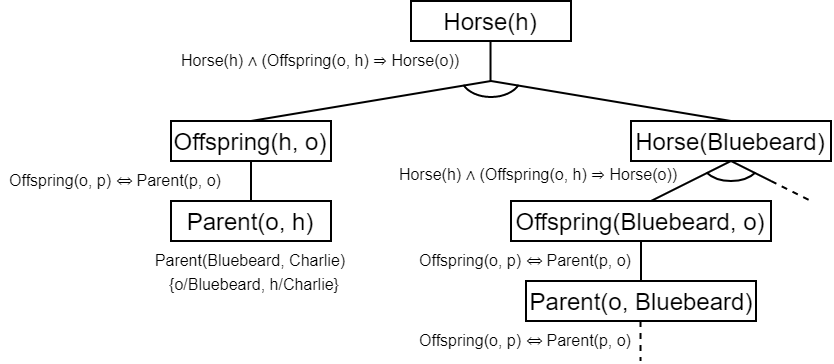
\includegraphics[scale=.6]{Pics/HW4_Q9-16.png}
\end{figure}\\[.4em]
\noindent 2) The domain extends forever, and because of that there are two infinite loops.\\[.4em]
\noindent 3) 2 solutions, Charlie and Bluebeard.\\[.4em]



\noindent \hrulefill \pagebreak



\centerline{- 9.18 - }
\ \\
\noindent 1) \begin{multicols}{2}
\hspace*{0pt}\hfill P(A, [1, 2, 3])\\
\hspace*{0pt}\hfill P(1, [1|2, 3])\\
\hspace*{0pt}\hfill P(1, [1|2, 3])\\
\hspace*{0pt}\hfill P(2, [2, 3])\\
\hspace*{0pt}\hfill P(2, [2, 3])\\
\hspace*{0pt}\hfill P(3, [3])\\
\hspace*{0pt}\hfill P(3, [3])\\
Goal\\
Solution with A=1\\\\
Solution with A=2\\\\
Solution with A=3\\
\end{multicols}

\noindent 2) \begin{multicols}{2}
\hspace*{0pt}\hfill P(2, [1, A, 3])\\
\hspace*{0pt}\hfill P(2, [1|2, 3])\\
\hspace*{0pt}\hfill P(2, [1|2, 3])\\
\hspace*{0pt}\hfill P(2, [2, 3])\\
\hspace*{0pt}\hfill P(2, [2, 3])\\
\hspace*{0pt}\hfill P(3, [3])\\
\hspace*{0pt}\hfill P(3, [3])\columnbreak\\
Goal\\\\\\
Solution with A=2\\
\end{multicols}



\noindent \hrulefill \\


\end{document}

















